%% LyX 2.3.6.1 created this file.  For more info, see http://www.lyx.org/.
%% Do not edit unless you really know what you are doing.
\documentclass[english]{article}
\usepackage[T1]{fontenc}
\usepackage[latin9]{inputenc}
\usepackage{geometry}
\geometry{verbose,tmargin=2.5cm,bmargin=2.5cm,lmargin=2.5cm,rmargin=2.5cm}
\usepackage{calc}
\usepackage{amsmath}
\usepackage{graphicx}

\makeatletter

%%%%%%%%%%%%%%%%%%%%%%%%%%%%%% LyX specific LaTeX commands.
%% Because html converters don't know tabularnewline
\providecommand{\tabularnewline}{\\}

\makeatother

\usepackage{babel}
\begin{document}
{[}SPLIT\_HERE{]}
\begin{enumerate}
\item \textbf{{[}RVHS/PRELIM/9597/2017/P1/Q1{]} }

\textbf{Results management }

For this task, you are required to read the text file \textquotedblleft \textbf{overall\_grades.txt}\textquotedblright{}
which contains the subject grades of the first and second semester
examination of 50 students.

The format of the text file is as follow: \texttt{<name>;<subject1>:<grade1>,<grade2>;<subject2>:<grade1>,<grade
2>;<subject3>:<grade1>,<grade2>,\dots etc;\textbackslash n }

For example: 

\texttt{Rufus Schuck;EL:C,B;CL:C,C;Math:C,E;Bio:B,F; }

Student Rufus Schuck takes 4 subjects. They are English (EL), Chinese
(CL), Math (Math) and Biology (Bio). His 1st and 2nd semester grades
for English is C and B respectively. 

\subsection*{Task 1.1 }

Write the program code for the function process\_data() which reads
the text file \textquotedblleft \textbf{overall\_grades.txt}\textquotedblright{}
and returns a dictionary which has the following format. 

\texttt{\{'Rufus Schuck': \{'EL': {[}'C', 'B'{]}, 'CL': {[}'C', 'C'{]},
'Math': {[}'C', 'E'{]}, 'Bio': {[}'B', 'F'{]}\}, ...\} }

The returned dictionary uses the name of student as key and another
dictionary as its return value. This \textquotedblleft another\textquotedblright{}
dictionary then uses the subjects and a list containing the grades
of the 1st and 2nd semesters as its key and value respectively. 

\subsection*{Evidence 1 }

The program code for the function \texttt{process\_data()}. \hfill{}{[}4{]}

\subsection*{Task 1.2}

Write a function \texttt{have\_n\_improvement(n)} which takes in an
integer \texttt{n} and returns a list of student names who have improvement
in exactly \texttt{n} subject(s). Using the example in Task 1.1, '\texttt{Rufus
Schuck}' shows improvement in only English. So, if \texttt{n} is 1,
'\texttt{Rufus Schuck}' must be included in the student name list. 

\subsection*{Evidence 2}

The program code for the function \texttt{have\_n\_improvement(n)}.\hfill{}
{[}3{]}

\subsection*{Task 1.3 }

Write a function \texttt{have\_improvement\_in\_all\_subjs()} which
returns a list of student names who have improvement in all his/her
subjects. 

\subsection*{Evidence 3}

The program code for the function have\_improvement\_in\_all\_subjs(n).\hfill{}
{[}3{]}

\subsection*{Task 1.4 }

Write a function \texttt{count\_combi(combi)} which takes a list of
subjects \texttt{combi} as input and returns the total number of students
who take the subject combination in \texttt{combi}. Take note that
students who take more subjects than what is indicated in \texttt{combi}
are included. 

For example:

\noindent\begin{minipage}[t]{1\columnwidth}%
\texttt{>\textcompwordmark >\textcompwordmark > count\_combi({[}'EL',
'MATH'{]}) }

\texttt{>\textcompwordmark >\textcompwordmark > 50 }%
\end{minipage}

\subsection*{Evidence 4 }

The program code for the function \texttt{count\_combi(n)}. \hfill{}{[}4{]}

\subsection*{Task 1.5}

Using your solution in Task 1.4, find the total number of students
who take \textquotedbl Chem\textquotedbl{} and \textquotedbl Bio\textquotedbl{}
but not \textquotedbl Physics\textquotedbl . 

\subsection*{Evidence 5 }

The program code to find what is required in Task 1.5. \hfill{}{[}2{]}

\subsection*{Task 1.6 }

Write a function \texttt{calculate\_GPA(name)} which takes a string
\texttt{name} as input and calculates the GPA of the student indicated
by \texttt{name}. 

The points for each grade are as follow: 

\texttt{\{'A':5, 'B':4, 'C':3, 'D':2, 'E':1, 'F':0\} }

The 1 st and 2nd semester grades in the data has the same weightages. 

To calculate GPA,
\begin{itemize}
\item Find the average points achieved of each subject.
\begin{itemize}
\item e.g. if a student gets C and D in \textquotedbl CL\textquotedbl ,
his average points for \textquotedbl CL\textquotedbl{} is 3 + 2 =
2.5 
\end{itemize}
\item Add up the average points of each subject 
\item Divide the total by the number subjects the student takes 
\begin{itemize}
\item e.g. \texttt{'Claudette Bode': \{'EL': {[}'C', 'D'{]}, 'CL': {[}'D',
'A'{]}, 'Math': {[}'A', 'D'{]}, 'Phy': {[}'A', 'D'{]}, 'Bio': {[}'D',
'C'{]}\}}, 
\item \texttt{{[}(3 + 2)/2 + (2 + 5)/2 + (5 + 2)/2 + (2 + 5)/2 + (2 + 3)/2{]}/5
= 3.1}
\end{itemize}
\item GPA for '\texttt{Claudette Bode}' is 3.1 
\end{itemize}

\subsection*{Evidence 6 }

The program code for the function \texttt{calculate\_GPA(name)}.\hfill{}
{[}4{]}

{[}SPLIT\_HERE{]}
\item \textbf{{[}RVHS/PRELIM/9597/2017/P1/Q2{]} }

\textbf{Missing phone number digits }

Your friend (Mary) made an oversea friend (Jenny) yesterday while
she was studying in the regional library. To remain in contact, Jenny
gave Marry her phone number and told Mary that it is also a valid
10 digits International Standard Book Number (ISBN). 

After Jenny had left, Mary accidentally punched a few holes on the
phone number while she was arranging her notes using the library\textquoteright s
hole puncher machine. It was too difficult for Mary to recover the
lost pieces of paper. So, Mary decided to look for you to recover
the missing digits instead. Below is the picture of the paper.
\noindent \begin{center}
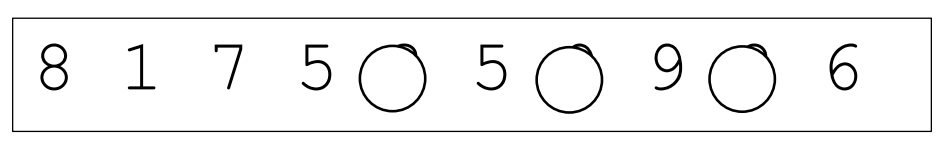
\includegraphics[width=0.5\paperwidth]{C:/Users/Admin/Desktop/Github/question_bank/LyX/static/img/9597-RHVS-2017-P1-Q1-1}
\par\end{center}

To recover the missing digits, you need to understand how ISBN-10
works. The steps to check for a valid ISBN-10 is as follow: 
\begin{enumerate}
\item[1.]  Each of the digits of the ISBN-10 is first multiplied by a number
in a sequence from 10 to 1 (Take note that the last digit of the ISBN-10
can be \textquoteleft X\textquoteright{} which holds a value of 10).
\item[2.]  All the 10 digits are then added up together. 
\item[3.]  If the sum is divisible by 11, it is a valid ISBN-10, else it is
invalid. 
\end{enumerate}
For example, to check if \textquoteleft 997150233X\textquoteright{}
is a valid ISBM-10:

\noindent %
\noindent\begin{minipage}[t]{1\columnwidth}%
\emph{Step 1 and 2}

\emph{
\begin{align*}
 & (9\times10)+(9\times9)+(7\times8)+(1\times7)+(5\times6)+(0\times5)+(2\times4)+(3\times3)+(3\times2)+(\boldsymbol{X}\times1)\\
= & (9\times10)+(9\times9)+(7\times8)+(1\times7)+(5\times6)+(0\times5)+(2\times4)+(3\times3)+(3\times2)+(\boldsymbol{10}\times1)\\
= & 297
\end{align*}
}

\emph{Step 3}

\emph{297 is a multiple of 11. Therefore, \textquoteleft 997150233X\textquoteright{}
is a valid ISBN-10. }%
\end{minipage}

\subsection*{Task 2.1}

Write a function \texttt{is\_valid\_ISBN10(isbn10)} which takes a
string \texttt{isbn10} as input and returns \texttt{True} if \texttt{isdn10}
is a valid ISBN-10 and \texttt{False} otherwise. You are to validate
the input string \texttt{isbn10} and print to terminal the issue related
to the \texttt{isbn10} string. The possible issues to be printed to
terminal includes:
\begin{itemize}
\item \texttt{ISBN-10 must only have 10 digits. }
\item \texttt{ISBN-10 can only contain numbers and the character 'X'. }
\item \texttt{'X' can only be found at the last digit of isbn10. }
\item \texttt{Wrong check digit.}
\item \texttt{Valid ISBN-10. }
\end{itemize}

\subsection*{Evidence 7 }

The program code for the function \texttt{is\_valid\_ISBN10(isbn10)}.
\hfill{}{[}6{]}

\subsection*{Task 2.2 }

Write a function \texttt{possible\_ISBN(isbn)} which takes a query
string \texttt{isbn10} as input and returns a list of possible ISBN-10.
The query string \texttt{isbn10} has 3 missing digits replaced with
a '\texttt{?}' and they can be at any positions of the query string. 

For example, 

\noindent %
\noindent\begin{minipage}[t]{1\columnwidth}%
\texttt{>\textcompwordmark >\textcompwordmark > possible\_ISBN(\textquotedbl 9971??23?X\textquotedbl ) }

\texttt{>\textcompwordmark >\textcompwordmark > {[}'997100237X',
'997102232X', '997103235X', '997104238X', '997105230X', '997106233X',
'997107236X', '997108239X', '997109231X', '997110234X', '997111237X',
'997113232X', '997114235X', '997115238X', '997116230X', '997117233X',
'997118236X', '997119239X', '997120231X', '997121234X', '997122237X',
'997124232X', '997125235X', '997126238X', '997127230X', '997128233X',
'997129236X', '997130239X', '997131231X', '997132234X', '997133237X',
'997135232X', '997136235X', '997137238X', '997138230X', '997139233X',
'997140236X', '997141239X', '997142231X', '997143234X', '997144237X',
'997146232X', '997147235X', '997148238X', '997149230X', '997150233X',
'997151236X', '997152239X', '997153231X', '997154234X', '997155237X',
'997157232X', '997158235X', '997159238X', '997160230X', '997161233X',
'997162236X', '997163239X', '997164231X', '997165234X', '997166237X',
'997168232X', '997169235X', '997170238X', '997171230X', '997172233X',
'997173236X', '997174239X', '997175231X', '997176234X', '997177237X',
'997179232X', '997180235X', '997181238X', '997182230X', '997183233X',
'997184236X', '997185239X', '997186231X', '997187234X', '997188237X',
'997190232X', '997191235X', '997192238X', '997193230X', '997194233X',
'997195236X', '997196239X', '997197231X', '997198234X', '997199237X'{]}}%
\end{minipage}

\subsection*{Evidence 8 }

The program code for the function \texttt{possible\_ISBN(isbn)}. \hfill{}{[}6{]}

\subsection*{Task 2.3}

Examine the missing numbers in the paper closely and eliminate impossible
digit choices. For example, the three missing digits cannot be \textquoteleft 1\textquoteright{}
as the three missing digits in the paper have round edges at the top.
Modify your solution in Task 2.2 and suggest these possible ISBN-10
to Mary.

\subsection*{Evidence 9 }

The screenshot of the suggested possible ISBN-10 that you will give
to Mary.\hfill{} {[}2{]}

\subsection*{Task 2.4 }

Write a menu to help other to generate possible ISBN-10. The menu
should have the following functions. 
\noindent \begin{center}
\begin{tabular}{|l|}
\hline 
\texttt{Menu}\tabularnewline
\texttt{A) Input a ISBN-10 query string}\tabularnewline
\texttt{B) Display all possible ISBN-10}\tabularnewline
\texttt{C) Quit}\tabularnewline
\hline 
\end{tabular}
\par\end{center}

You should validate user inputs and call for re-entry when an invalid
option is given. 

\subsection*{Evidence 10}

Program code for the procedure \texttt{menu()}.\hfill{} {[}6{]}

{[}SPLIT\_HERE{]}
\item \textbf{{[}RVHS/PRELIM/9597/2017/P1/Q3{]} }

\textbf{Unsorted Linked List}

The classes Node and LinkedList is partially implemented for you according
to the specification given below. The attribute start of class LinkedList
stores the first node instance of the linked list. If the linked list
has no node, start has the value of None. Functions in bold are not
implemented. 
\begin{center}
\texttt{}%
\begin{tabular}{|l|}
\hline 
\texttt{\hspace{0.25\columnwidth}Node}\tabularnewline
\hline 
\texttt{-data : STRING}\tabularnewline
\texttt{-next : Node}\tabularnewline
\hline 
\texttt{+constructor()}\tabularnewline
\texttt{+set\_data(data)}\tabularnewline
\texttt{+get\_data()}\tabularnewline
\texttt{+set\_next(node)}\tabularnewline
\texttt{+get\_next()}\tabularnewline
\texttt{+\_\_str\_\_()}\tabularnewline
\hline 
\end{tabular}\texttt{}%
\begin{tabular}{|l|}
\hline 
\texttt{\hspace{0.25\columnwidth}LinkedList}\tabularnewline
\hline 
\texttt{-start : Node}\tabularnewline
\tabularnewline
\hline 
\texttt{+constructor()}\tabularnewline
\texttt{+set\_start(node)}\tabularnewline
\texttt{+get\_start()}\tabularnewline
\texttt{\textbf{+insert\_data(data)}}\tabularnewline
\texttt{\textbf{+transfer(linkedlist)}}\tabularnewline
\texttt{\textbf{+delete\_pos(pos)}}\tabularnewline
\texttt{+display() }\tabularnewline
\hline 
\end{tabular}
\par\end{center}

\subsection*{Task 3}

Implement the following \texttt{LinkedList} class functions according
to its specification given: 
\begin{itemize}
\item \texttt{+insert\_data(data) : }This function takes a string \texttt{data}
as input and uses its value to create a new \texttt{Node} instance.
The new Node instance is then inserted as the first node of the linked
list\texttt{.}
\item \texttt{+transfer(llist) :} This function takes a \texttt{LinkedList}
instance \texttt{llist} as input and transfers all its \texttt{Node}
instances in the same order to the \texttt{LinkedList} instance that
calls for this function. 

For example: 

\noindent\begin{minipage}[t]{1\columnwidth}%
\texttt{A:'boy'->'man'->'woman'}

\texttt{B:'girl'->'baby' }

\texttt{>\textcompwordmark >\textcompwordmark > A.transfer(B) }

\texttt{A: 'boy'->'man'->'woman'->'girl'->'baby'}

\texttt{B: None}%
\end{minipage}
\item \texttt{+delete\_pos(pos) : }This function takes in an integer pos
as input and deletes the node at position pos. Take note that the
first node of the linked list is position 1.

For example: 

\noindent\begin{minipage}[t]{1\columnwidth}%
\texttt{A:'boy'->'man'->'woman' }

\texttt{>\textcompwordmark >\textcompwordmark > A. delete\_pos(2) }

\texttt{A:'boy'->'woman'}%
\end{minipage}
\end{itemize}

\subsection*{Evidence 11 }

Program code for: 
\begin{itemize}
\item \texttt{insert\_data(node)} \hfill{}{[}3{]}
\item \texttt{transfer(linkedlist) }\hfill{}{[}3{]}
\item \texttt{delete\_pos()}\hfill{} {[}4{]}
\end{itemize}
{[}SPLIT\_HERE{]}
\item \textbf{{[}RVHS/PRELIM/9597/2017/P1/Q4{]} }

\textbf{Sorting Algorithms }

The pseudocode procedure below is given a list of integers in random
order, the procedure then outputs a sorted list in ascending order. 

\noindent\fbox{\begin{minipage}[t]{1\columnwidth - 2\fboxsep - 2\fboxrule}%
\texttt{01. FUNCTION Merge\_Sort (ARRAY: arr) }

\texttt{02. \qquad{}n = SIZE(arr) }

\texttt{03. \qquad{}IF n < 2: }

\texttt{04. \qquad{}\qquad{}RETURN arr }

\texttt{05. \qquad{}END IF }

\texttt{06. \qquad{}left = Merge\_Sort(PARTITION(arr, 0, n DIV 2)) }

\texttt{07. \qquad{}right = Merge\_Sort(PARTITION(arr, n DIV 2, n)) }

\texttt{08. \qquad{}RETURN Merge(left, right) }

\texttt{09. END FUNCTION }

\texttt{10.}

\texttt{11. FUNCTION Merge (ARRAY: left, LIST: right) }

\texttt{12. \qquad{}DECLARE results: ARRAY{[}SIZE(left) + SIZE(right){]} }

\texttt{13. \qquad{}DECLARE i, j, index : INTEGER }

\texttt{14. \qquad{}i, j, index = 0, 0, 0 }

\texttt{15. \qquad{}WHILE i < SIZE(left) and j < SIZE(right)}

\texttt{16. \qquad{}\qquad{}IF left{[}i{]} < right{[}j{]}:}

\texttt{17. \qquad{}\qquad{}\qquad{}results{[}index{]} = left{[}i{]} }

\texttt{18. \qquad{}\qquad{}\qquad{}i = i + 1}

\texttt{19. \qquad{}\qquad{}ELSE: }

\texttt{20. \qquad{}\qquad{}\qquad{}results{[}index{]} = right{[}j{]}}

\texttt{21. \qquad{}\qquad{}\qquad{}j = j + 1}

\texttt{22. \qquad{}\qquad{}END IF }

\texttt{23. \qquad{}\qquad{}index = index + 1 }

\texttt{24. \qquad{}END WHILE}

\texttt{25. \qquad{}WHILE i < SIZE(left)}

\texttt{26. \qquad{}\qquad{}results{[}index{]} = left{[}i{]} }

\texttt{27. \qquad{}\qquad{}i = i + 1}

\texttt{28. \qquad{}\qquad{}index = index + 1 }

\texttt{29. \qquad{}END WHILE}

\texttt{30. \qquad{}WHILE j < SIZE(right) }

\texttt{31. \qquad{}\qquad{}results{[}index{]} = right{[}j{]} }

\texttt{32. \qquad{}\qquad{}j = j + 1 }

\texttt{33. \qquad{}\qquad{}index = index + 1 }

\texttt{34. \qquad{}END WHILE}

\texttt{35. \qquad{}RETURN results}

\texttt{36. END FUNCTION }%
\end{minipage}}

\subsection*{Task 4.1 }

Write program code to implement the given procedure. Execute the function
using the following list as the parameter. 

\texttt{{[}1, 15, 2, 4, 3, 9, 7, 10{]}} 

\subsection*{Evidence 12 }

Program Code. Screenshot showing the output. \hfill{}{[}6{]}

\subsection*{Evidence 13}

Analyze and state the time complexity of the algorithm in big $O$
notation.\hfill{} {[}1{]}

\subsection*{Task 4.2 }

Bubble sort is a common sorting algorithm, below is an implementation
of in-place bubble sort using recursion. There are three missing lines
in the pseudocode, indicated as \texttt{A}, \texttt{B} and \texttt{C}. 

\noindent\fbox{\begin{minipage}[t]{1\columnwidth - 2\fboxsep - 2\fboxrule}%
\texttt{01. PROCEDURE Bubble\_Sort (ARRAY: arr, INTEGER: n) }

\texttt{02. \qquad{}IF \_\_\_\_\_\_\_A\_\_\_\_\_\_\_:}

\texttt{03. \qquad{}\qquad{}RETURN }

\texttt{04. \qquad{}END IF }

\texttt{05. }

\texttt{06. \qquad{}FOR i FROM 0 TO (n-1): }

\texttt{07. \qquad{}\qquad{}IF \_\_\_\_\_\_\_B\_\_\_\_\_\_\_: }

\texttt{08. \qquad{}\qquad{}\qquad{}temp = arr{[}i{]} }

\texttt{09. \qquad{}\qquad{}\qquad{}arr{[}i{]} = arr{[}i+1{]} }

\texttt{10. \qquad{}\qquad{}\qquad{}arr{[}i+1{]} = temp }

\texttt{11. \qquad{}\qquad{}END IF }

\texttt{12. \qquad{}END FOR }

\texttt{13.}

\texttt{14. \qquad{}\_\_\_\_\_\_\_C\_\_\_\_\_\_\_ }

\texttt{15. END PROCEDURE }%
\end{minipage}}

Execute the procedure to sort the following list. \texttt{{[}1, 15,
2, 4, 3, 9, 7, 10{]} }

\subsection*{Evidence 14}

Complete the missing lines \texttt{A}, \texttt{B} and \texttt{C}.
\hfill{}{[}3{]}

Insert a counting mechanism to count the number of comparisons made,
and return the value as an integer. Implement the new recursive bubble
sort. 

\subsection*{Evidence 15}

Program Code. 

Screenshot showing the output of the sorted list and count value.
\hfill{}{[}4{]}

\subsection*{Evidence 16 }

Analyze and state the time complexity of the algorithm in big $O$
notation. \hfill{} {[}1{]}

\subsection*{Task 4.3}

Due to the nature of bubble sort, if no swaps are observed in a given
iteration, then there is no need for the next iteration. Implement
the improved bubble sort. Execute the function to sort the following
list.

\texttt{{[}1, 15, 2, 4, 3, 9, 7, 10{]}}

\subsection*{Evidence 17}

Program Code. Screenshot showing the output of the sorted list and
count value. \hfill{}{[}3{]}

{[}SPLIT\_HERE{]}
\item \textbf{{[}RVHS/PRELIM/9597/2017/P1/Q5{]} }

\textbf{Grocery Store Manager }

The grocery shop in the neighborhood ask your help to create an application
to manage the grocery store. 

First, you are tasked to work on an object-oriented solution to store
all the grocery details. The \texttt{title} of the grocery item, \texttt{cost},
\texttt{price} and \texttt{stock} of each grocery is recorded. Besides
the normal groceries, the shop identifies three unique types of grocery
too, namely:
\begin{itemize}
\item Electrical Appliance: there is a need to indicate the \texttt{power}
of the product to understand its energy consumption rate.
\item Cigarette: it is important to track the \texttt{nicotine content}
of various kinds of cigarette.
\item Alcohol: there are distinct \texttt{types} of alcohols such as wine
or beer. 
\end{itemize}
Below is an UML class diagram for your reference. 

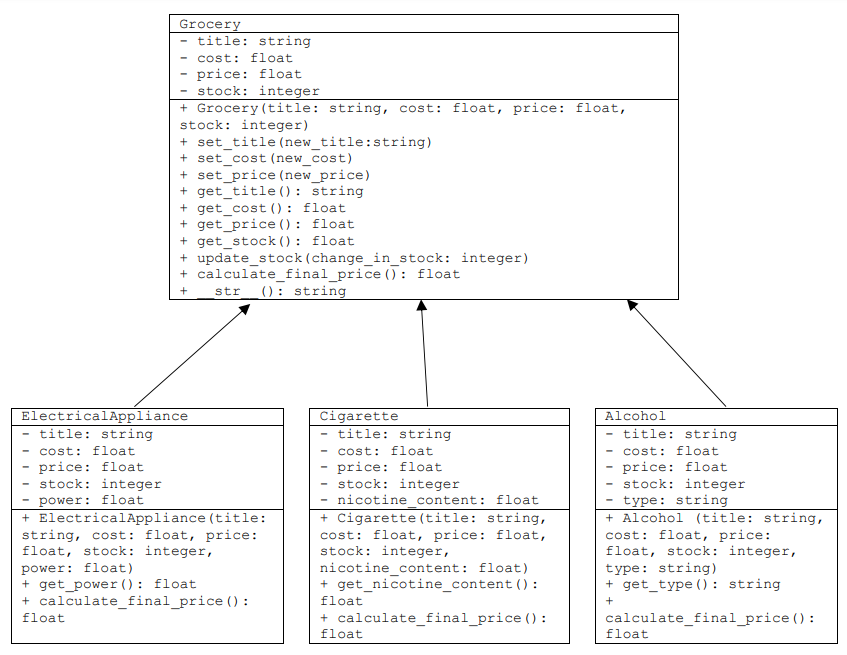
\includegraphics[width=0.65\paperwidth]{C:/Users/Admin/Desktop/Github/question_bank/LyX/static/img/9597-RVHS-2017-P1-Q5-1}

\subsection*{Task 5.1}

Implement the classes of \texttt{Grocery}, \texttt{ElectricalAppliance},
\texttt{Cigarette} and \texttt{Alcohol} with object-oriented programming.

\subsection*{Evidence 18}

Program Code for four classes. \hfill{}{[}7{]}

\subsection*{Task 5.2 }

In country S, purchasing all groceries will incur a 7\% Goods and
Services Tax(GST). 

To promote healthy living, additional tax have been imposed to cigarettes
and alcohols: 
\begin{itemize}
\item Cigarette: additional 60\% tax 
\item Wines: additional 50\% tax 
\item Beers: additional 20\% tax 
\end{itemize}
For example: \emph{the price of one packet of \textquotedblleft Yun
Yan\textquotedblright{} cigarette is \$23.00, the final price can
be calculated by: \$23.00 x 160\% x 107\% = \$39.38}

In addition, to support the \textquotedblleft save energy movement\textquotedblright ,
all electrical appliance with a power less than or equals to 10Watt
was set to be sold at 80\% of its original price. 

Implement the function \texttt{calculate\_final\_price()} which includes
the above mentioned tax and promotion into consideration. 

Implement the \texttt{\_\_str\_\_()} function which returns a string
in the following format (You may refer to the \texttt{test\_function\_5\_1()}
to understand the formatting): 

\texttt{Title | Cost | Price | Stock | Final Price }

For example, Yun Yan\textquoteright s cost is \$16.50, price is set
at \$23.00, the current stock is 4 and final price is \$39.38. The
\_\_str\_\_() function should return the following string:

\texttt{Yun Yan | \$ 16.50 | \$ 23.00 | 4 | \$ 39.38}

\subsection*{Evidence 19 }

Program Code for \texttt{calculate\_final\_price()} and \texttt{\_\_str\_\_()}. 

Screenshot showing output of \texttt{test\_function\_5\_1()}. \hfill{}{[}6{]}

\subsection*{Task 5.3}

Implement a class \texttt{StoreManager} which keep track of a list
of grocery items, \texttt{curr\_item\_list}. The \texttt{StoreManager}
should have the following class functions: 
\begin{itemize}
\item \texttt{sell\_item(sold\_item)} \texttt{sold\_item} is a tuple containing
2 elements: the \texttt{title} of the item and the \texttt{quantity}
sold. You may assume the title of item is always valid and the quantity
sold is always smaller than the current stock. 

The function should decrease the current stock of the sold items.
Upon completion, it should print out a string containing the following
information:

\texttt{Title | Unit Price | Quantity Sold | Subtotal}

The function should return a float containing the \texttt{sub\_total}
value.
\item \texttt{sell\_items(sold\_item \_list)} \texttt{sold\_item\_list}
is a list of tuples; each tuple containing the item \texttt{title}
and \texttt{quantity} sold. 

The function should print out a table displaying information for all
sold items in the following format: 

\texttt{Title | Unit Price | Quantity Sold | Subtotal}

The summary should end with a line indicating the overall total value
of items sold in this transaction. 
\item \texttt{stock\_check()} When this function is called, it should check
the list of all grocery items and print out a summary of items with
current stock value below 5. This indicates the need for stocking
up these items soon. A summary table should be printed in the following
format: 

\texttt{Title | Unit Cost | Quantity Left }
\end{itemize}

\subsection*{Evidence 20 }

Program Code for class functions of StoreManager class: 
\begin{itemize}
\item sell\_item \hfill{}{[}3{]}
\item sell\_items \hfill{}{[}2{]}
\item stock\_check \hfill{}{[}2{]}
\end{itemize}
Screenshot showing output of \texttt{test\_function\_5\_2()}.\hfill{}
{[}2{]}

{[}SPLIT\_HERE{]}
\end{enumerate}

\end{document}
